\documentclass[12pt]{article}
\usepackage{array}
\usepackage{amsmath}
\usepackage{mathtools}
\usepackage{gensymb}
\usepackage{graphicx}
\usepackage{float}
\usepackage{caption}
\usepackage{setspace}


\allowdisplaybreaks

\begin{document}
    \setstretch{1.25}
    \title{Density of Water}
    \author{Ryan Coyne, Ben Eid, Erin Snook}
    \maketitle
    \section{Abstract}
        The density of water was measured using the volume and mass of the water in Part I and by using Archimedes principle in Part II. The value for the density of water found in Part I was (1013 \(\pm\) 48) \(\mathrm{kg/m^3}\) and was \((1010 \pm 58 \mathrm{kg/m^3})\). Part I was done individually and Part II was done as a group.
    \section{Introduction}
        The density of a material is the ammount of mass of that material contained in a unit of volume. From just that definition we know that density can be calculated from a known mass and volume by dividing the value of the mass by the value of the volume. For fluids, it is also possible to use Archimedes principle to determine the density of the fluid in question. 

        Archimedes principle says that the bouyant force on an object is equal to the weight of the fluid displaced by that object. The wight of the object is equal to it's mass times the acceleration due to gravity and mass is density times volume. As a result Archimedes principle can be reprsented as
        \begin{equation*}
            F_b = \rho g V
        \end{equation*}
        where \(F_b\) is the bouyant force on the object, \(\rho\) is the density of the fluid, \(g\) is the acceleration due to gravity, and \(V\) is the volume of the object.

        When the bouyant force on a completely submerged object is plotted against the volume of that object, then the slope of the line of best fit is \(\rho \text{ times } g\). With a known \(g\) and a known slope, \(\rho\) can be found by dividing the slope by \(g\).
    \section{Procedure}
        \subsection*{Part I}
        Set out a tripple beam balance and a 100 mL graduated cylinder. Measure the mass of the graduated cylinder three times using the tripple beam balance. Add 100 mL of tap water to the graduated cylinder. Measure the mass of the newly filled graduated cylinder three times using the tripple beam balance. 
        \subsection*{Part II}
        Acquire two metal rods, a c-clamp with a slot to hold a rod, an angle clamp witch can hold two clamps at a right angle to one another, an electronic force sensor from which objects can be hung, a string, three objects of various volumes, and a bowl that is large enough to submerge all three objects. 
        
        Attach the c-clamp to a table and fit one rod into the clamp so that it is vertical. Attach the angle clamp to the vertical rod and insert the second rod so that it is horrizontal. Attach the force sensor to the horrizontal rod so that it is above the table, and connect it to a recording device. Hang a string from the force sensor. Fill the bowl with enough water to completely submerge all of the objects. For one object at a time, tie each object to the string so that it hangs above the table but lower than the surface of the water in the bowl. Allow the water to come to rest, and then record the weight of the object in air, and then when submerged in the water.\\
        \begin{figure}[H]
            \centering
            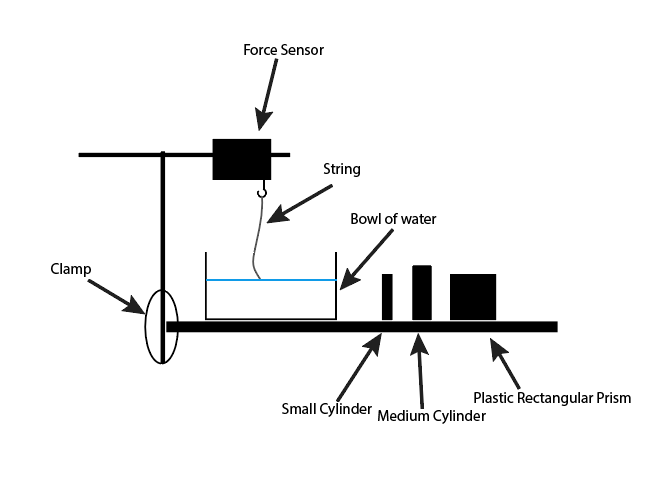
\includegraphics[width=0.75\linewidth]{setup.png}
            \caption{Experimental Setup}
        \end{figure}
    \section{Data}
    \subsection*{Part I}
        \begin{center}
            \begin{tabular}{c|c|c|c}
                Trial & \(m_c\) (g) & \(m_{cw}\) (g) & \(V\) (mL)\\
                \hline
                1 & 111.75 & 213.02 & 100\\
                2 & 111.89 & 213.10 & \\
                3 & 111.78 & 213.19 & \\
                \hline
                \(\overline{x}\) & 111.808 & 213.103 & 100\\
                \(\sigma\) & 0.074 & 0.085 & 5
            \end{tabular}\\[6pt]
            Table 1: Density of Water\\[12pt]
        \end{center}
        \subsection*{Part II}
        \begin{center}
            \begin{tabular}{c|c|c|c}
                \(d\) (cm) & \(h\) (cm) & \(W_d\) (N) & \(W_w\) (N)\\
                \hline
                1.262 & 5.010 & 0.569 & 0.505\\
            \end{tabular}\\[6pt]
            Table 2: Small Metal Cylinder\\[12pt]
            \begin{tabular}{c|c|c|c}
                \(d\) (cm) & \(h\) (cm) & \(W_d\) (N) & \(W_w\) (N)\\
                \hline
                2.473 & 5.039 & 0.659 & 0.418
            \end{tabular}\\[6pt]
            Table 3: Large Metal Cylinder\\[12pt]
            \begin{tabular}{c|c|c|c|c}
                \(l\) (cm) & \(w\) (cm) & \(h\) (cm) & \(W_d\) (N) & \(W_w\) (N)\\
                \hline
                2.533 & 2.528 & 2.532 & 0.200 & 0.029
            \end{tabular}\\[6pt]
            Table 4: Plastic Cube
        \end{center}
        \begin{figure}[H]
            \centering
            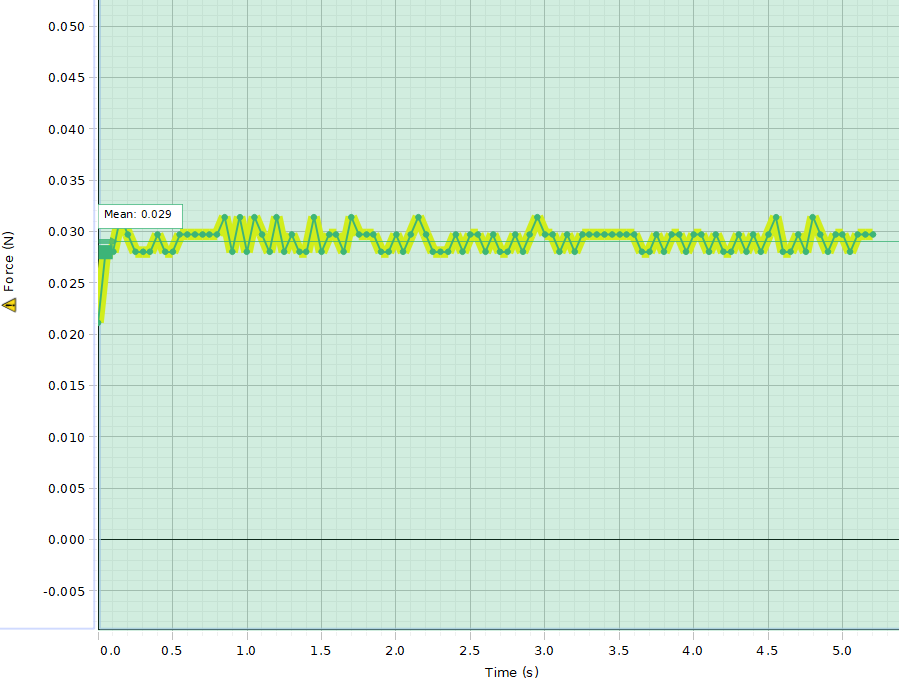
\includegraphics[width=0.75\linewidth]{force_time.png}
            \caption{Sample Plot of Force vs Time}
        \end{figure}
        \begin{figure}[H]
            \centering
            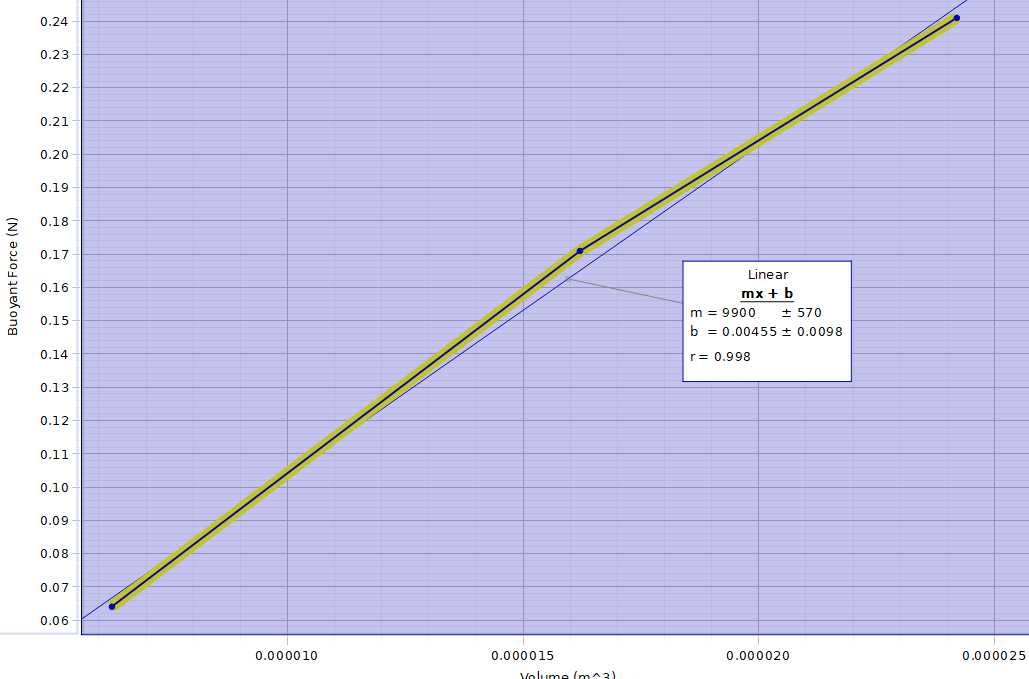
\includegraphics[width=0.75\linewidth]{linear_fit.png}
            \caption{Plot of Bouyant Force vs Volume with Linear Fit}
        \end{figure}
    \section{Calculations}
        \subsection*{Part I}
        \begin{alignat*}{3}
            (1)~&&
            \overline{\rho} &= \frac{\overline{m}_{cw}-\overline{m}_c}{\overline{V}}\\
            &&&=\frac{213.103 \text{ g} - 111.808 \text{ g} }{100 \text{ mL}}\\
            &&&=1.013 \mathrm{~g/cm^3}\\
            (2)~&&
            \text{Relative Error on } m_c &= \frac{0.074}{111.808}\\
            &&& = 0.066\%\\
            &&\text{Relative Error on } m_{cw} &=\frac{0.085}{213.103}\\ 
            &&&= 0.040\%\\
            &&\text{Relative Error on } V &=\frac{5}{100}\\
            &&& = 5\%\\
            (3)~&&
            \rho_V &= \frac{\overline{m}_{cw}-\overline{m}_c}{\overline{V+\sigma_V}}\\
            &&&=\frac{213.103-111.808}{105}\\
            &&&=0.964\\
            &&\sigma_\rho &= \sqrt{(\rho_v-\rho)^2}\\
            &&&=\sqrt{(0.964-1.013)^2}\\
            &&&=0.048
        \end{alignat*}
        \subsection*{Part II}
        \begin{alignat*}{3}
            (4)~&&
            V_{sc} &= \pi r^2h\\
            &&&=\pi\left(\frac{1.262\text{ cm}}{2}\right)^2(5.010\text{ cm})\\
            &&& = 6.27\mathrm{~cm^3}\\
            &&V_{lc} &= \pi\left(\frac{2.473\text{ cm}}{2}\right)^2(5.039\text{ cm})\\
            &&&=24.20\mathrm{~cm^3}\\
            &&V_\text{cube} &= lwh\\
            &&& = 2.533\text{ cm} \cdot 2.528\text{ cm} \cdot 2.532\text{ cm}\\
            &&& = 16.21\text{ cm}^3\\
            (5)~&&
            F_b&=\rho gV\\
            &&\rho g &= (9900 \pm 570)\mathrm{~N/m^3}\\
            && \overline{\rho} &= \frac{9900\mathrm{~N/m^3}}{9.8\mathrm{~m/s^2}}\\
            &&&=1010 \mathrm{~kg/m^3}\\
            (6)~&&
            \rho_{\rho g} &= \frac{(9900 + 570)\mathrm{~N/m^3}}{9.8\mathrm{~m/s^2}}\\
            &&&= 1068.37\mathrm{~kg/m^3}\\
            &&\sigma_\rho &= \sqrt{(1068.37\mathrm{~kg/m^3}-1010 \mathrm{~kg/m^3})^2}\\
            &&&= 58 \mathrm{~kg/m^3}\\
        \end{alignat*}
    \section{Conclusion}
        The density of water was measured to be (1013 \(\pm\) 48) \(\mathrm{kg/m^3}\) in using the mass-volume method, and \((1010 \pm 58 \mathrm{kg/m^3})\) using Archimedes principle. Both of these values are within one standard deviation of the expected value, \(1000 \mathrm{kg/m^3}\). The volume of water used was only measured once which could have introduced additional error. Allowing the water more time to come to rest in part 2 may also improve the results.
\end{document}